% =============================================================================
% CHAPITRE 4 -- RESULTATS, VALIDATION ET BILAN
% =============================================================================

\chapter{Résultats, validation et bilan}
\label{chap:resultats_validation_bilan}

Ce chapitre présente les résultats obtenus. Il ne
reprend pas le détail de chaque développement, déjà présenté dans le chapitre
précédent. Il met plutôt en évidence la manière dont les traitements ont été
validés, les formats couverts, les limites rencontrées et les apports de la
mission.


% =============================================================================
% 4.1 RESULTATS OBTENUS
% =============================================================================

\section{Résultats obtenus}
\label{sec:resultats_obtenus}

Les résultats peuvent être présentés selon les trois traitements principaux de
Scan : le \textit{listing}, le \textit{lookup} et la signature.

Les captures d'écran insérées dans cette section permettent d'illustrer les
sorties produites pour quelques formats représentatifs. Elles montrent à la
fois la structure des résultats et la manière dont les informations sont
retournées à Scan.

\begin{table}[H]
\centering
\renewcommand{\arraystretch}{1.25}
\begin{tabularx}{\textwidth}{>{\bfseries}p{3cm}X p{4.4cm}}
\toprule
\TableHeader Traitement & Résultat attendu & Exemples de formats concernés \\
\midrule
Listing &
Recenser les ressources accessibles dans un fichier ou une base de données. &
GeoPackage, Oracle, SQL Server. \\
\TableAlt Lookup &
Extraire les métadonnées nécessaires à la création ou à la mise à jour des
fiches. &
Rasters, vecteurs, GeoPackage, GeoParquet, CAO, Oracle, SQL Server. \\
Signature &
Produire une empreinte permettant de détecter les changements sur une donnée. &
GeoPackage, Oracle, SQL Server. \\
\bottomrule
\end{tabularx}
\caption{Synthèse des résultats selon les traitements de Scan}
\label{tab:resultats_par_traitement}
\end{table}

\subsection{Résultats du listing}
\label{subsec:resultats_listing}

Le listing correspond à l'inventaire des ressources accessibles. Il permet à
Scan d'identifier ce qui peut ensuite être documenté ou signé. Selon le format, le résultat peut correspondre à une liste de couches, de
tables ou de ressources présentes dans une connexion.

Pour GeoPackage, le listing devait parcourir le fichier et identifier les
couches disponibles.

Pour les bases Oracle et SQL Server, le listing devait récupérer toutes les tables auxquelles l'utilisateur a accès selon les paramètres de connexion utilisés.

\begin{figure}[H]
\centering
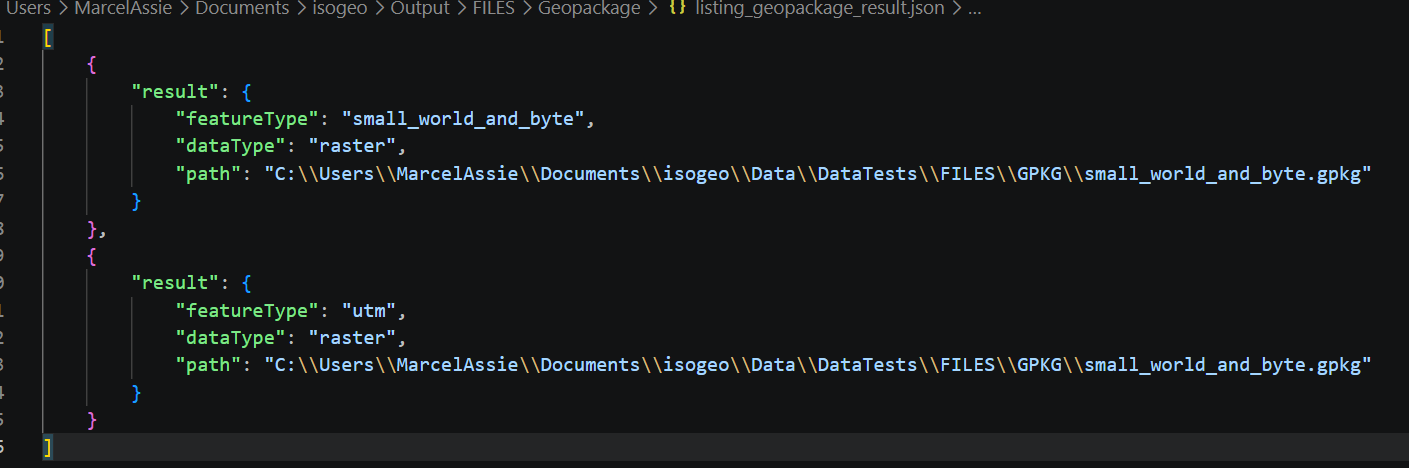
\includegraphics[width=\textwidth]{figures/isogeo/listing_geopackage.png}
\caption{Exemple de résultat de listing pour un fichier GeoPackage}
\label{fig:resultat_listing_geopackage}
\end{figure}

\begin{figure}[H]
\centering
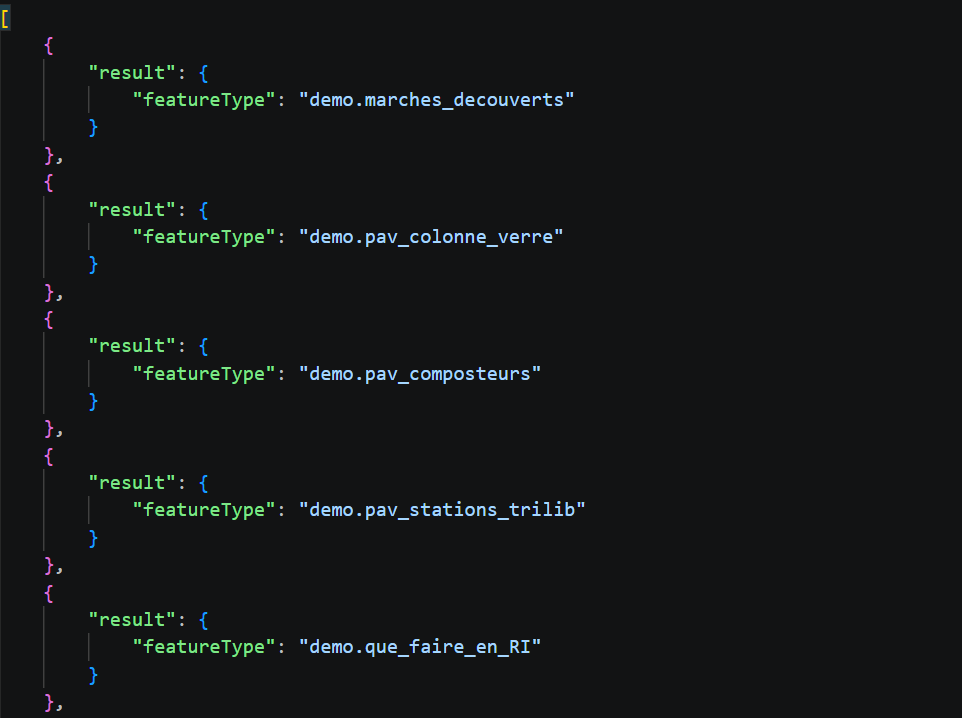
\includegraphics[width=\textwidth]{figures/isogeo/listing_sqlserver.png}
\caption{Exemple de résultat de listing pour une base de données SQL Server}
\label{fig:resultat_listing_sqlserver}
\end{figure}

\subsection{Résultats du lookup}
\label{subsec:resultats_lookup}


Les résultats obtenus varient selon la nature de la donnée. Pour les formats
vectoriels, le lookup permet de récupérer le nom, le format, le chemin, le
système de coordonnées, le type de géométrie, le nombre d'entités, les champs et
l'enveloppe convexe. Pour les rasters, il permet aussi de récupérer les
dimensions de l'image, le nombre de bandes et les propriétés associées aux
bandes.

Le lookup a également été adapté à des formats plus particuliers. Pour
GeoPackage, le traitement devait s'adapter au type de couche rencontré. Pour
GeoParquet. Pour les données CAO, on a lister toutes les couches du fichier devaient figurées
dans les métadonnées.

\begin{figure}[H]
\centering
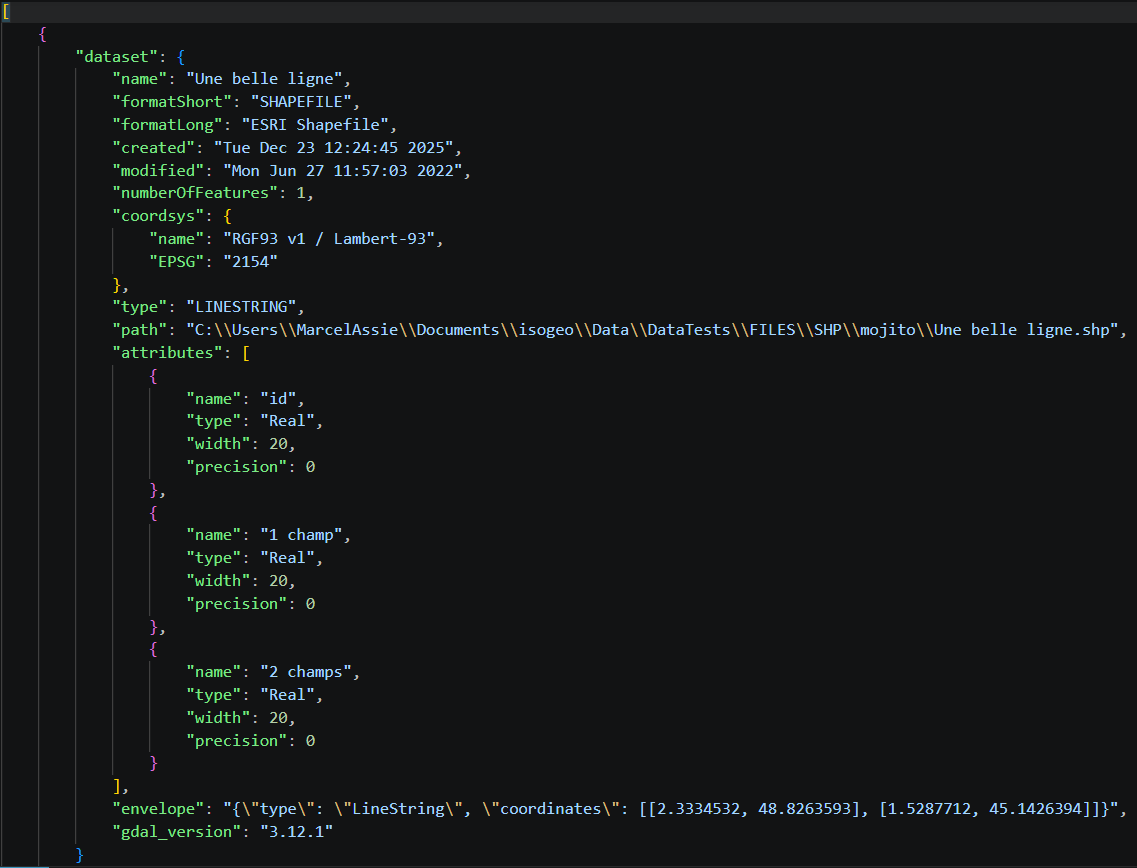
\includegraphics[width=\textwidth]{figures/isogeo/lookup_shapefile.png}
\caption{Exemple de résultat de lookup pour un fichier Shapefile}
\label{fig:resultat_lookup_shapefile}
\end{figure}

\begin{figure}[H]
\centering
\begin{subfigure}[t]{0.82\textwidth}
\centering
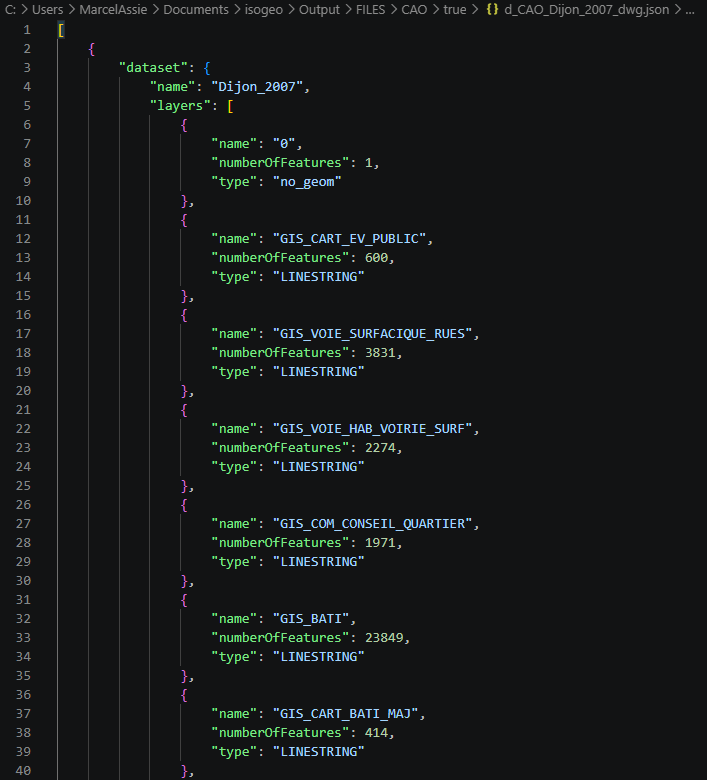
\includegraphics[width=\textwidth]{figures/isogeo/lookup_cao1.png}
\caption{Première partie du lookup d'un fichier DWG}
\label{fig:resultat_lookup_dwg_1}
\end{subfigure}

\medskip

\begin{subfigure}[t]{0.82\textwidth}
\centering
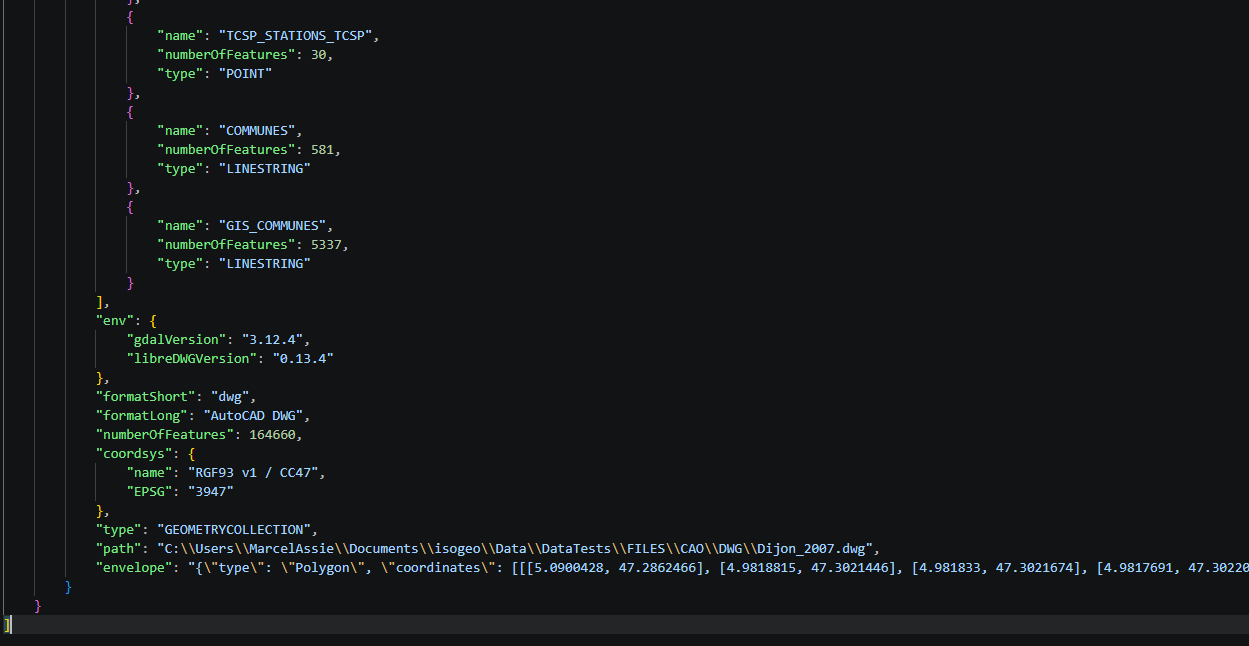
\includegraphics[width=\textwidth]{figures/isogeo/lookup_cao2.png}
\caption{Suite du lookup du même fichier DWG}
\label{fig:resultat_lookup_dwg_2}
\end{subfigure}
\caption{Exemple de résultat de lookup pour une donnée CAO au format DWG}
\label{fig:resultat_lookup_dwg}
\end{figure}

\subsection{Résultats de la signature}
\label{subsec:resultats_signature}

Le résultat de sortie d'une signature n'est pas une métadonnée descriptive, mais
une valeur de contrôle. Cette valeur doit rester stable si la donnée ne change
pas et évoluer lorsqu'une modification significative est apportée.

Les captures retenues permettent de montrer trois situations différentes. Pour
une donnée géographique, la clé \texttt{is\_geo} prend la valeur \texttt{1}. Pour
une donnée non géographique, elle prend la valeur \texttt{0}. Enfin, lorsqu'une
donnée ne contient aucune entité, la clé \texttt{is\_geo} reste à \texttt{null}
et une erreur est remontée. Ces cas sont importants, car ils ne produisent pas
exactement le même type de résultat.

\begin{figure}[H]
\centering
\begin{subfigure}[t]{0.48\textwidth}
\centering
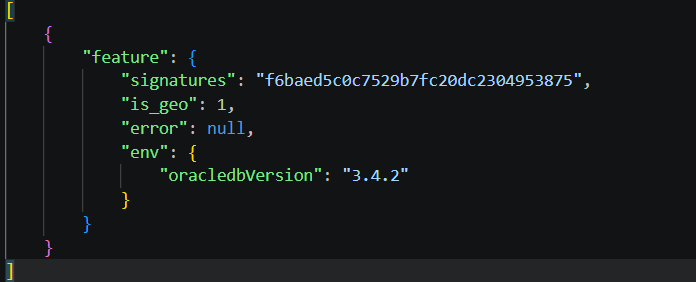
\includegraphics[width=\textwidth]{figures/isogeo/sign_donnee_geo.png}
\caption{Signature d'une donnée géographique}
\label{fig:resultat_signature_donnee_geographique}
\end{subfigure}
\hfill
\begin{subfigure}[t]{0.48\textwidth}
\centering
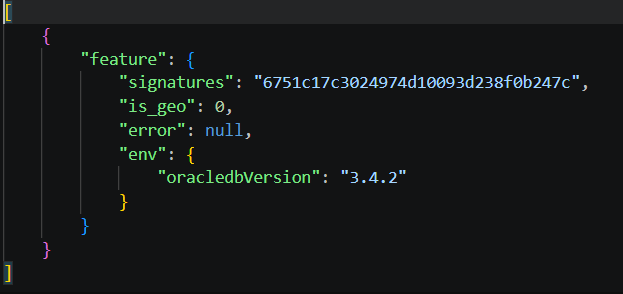
\includegraphics[width=\textwidth]{figures/isogeo/sign_donnee_non_geo.png}
\caption{Signature d'une donnée non géographique}
\label{fig:resultat_signature_donnee_non_geographique}
\end{subfigure}

\medskip

\begin{subfigure}[t]{0.62\textwidth}
\centering
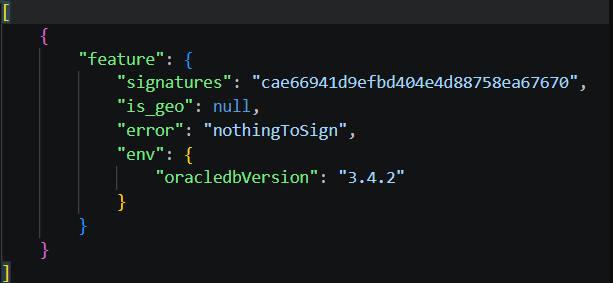
\includegraphics[width=\textwidth]{figures/isogeo/sign_donnes_san_entite.png}
\caption{Signature d'une donnée sans entité}
\label{fig:resultat_signature_donnee_sans_entite}
\end{subfigure}
\caption{Exemples de résultats de signature selon le type de donnée}
\label{fig:resultats_signature}
\end{figure}

% =============================================================================
% 4.2 VALIDATION DES TRAITEMENTS DEVELOPPES
% =============================================================================

\section{Validation des traitements développés}
\label{sec:validation_traitements_developpes}

La validation occupait une place importante dans la mission. La migration ne
consistait pas seulement à réécrire des traitements en Python. Il fallait aussi
montrer que les résultats produits étaient fiables, cohérents et exploitables
par Scan.

Pour rappel, trois familles de tests ont été utilisées : les tests de non-régression, les
tests d'intégrité de la signature et les tests de performance.

\begin{table}[H]
\centering
\renewcommand{\arraystretch}{1.25}
\begin{tabularx}{\textwidth}{>{\bfseries}p{3.2cm}X p{4.4cm}}
\toprule
\TableHeader Type de test & Objectif & Traitements concernés \\
\midrule
Non-régression &
Comparer les sorties Python avec les résultats de référence produits par les
anciens traitements. &
Inventaire et documentation. \\
\TableAlt Intégrité de la signature &
Vérifier que l'empreinte calculée réagit correctement aux modifications de la
donnée. &
Signature. \\
Performance &
Mesurer le comportement des scripts sur des volumes de données importants. &
Inventaire, documentation et signature. \\
\bottomrule
\end{tabularx}
\caption{Principales familles de tests utilisées pour valider les traitements}
\label{tab:tests_validation_chapitre_4}
\end{table}

\subsection{Tests de non-régression}
\label{subsec:tests_non_regression_chapitre_4}

Les tests de non-régression concernaient principalement le listing (recensessement) et le lookup (la documentation).
Ils consistaient à comparer les résultats produits par les
nouveaux scripts Python avec les résultats issus des traitements FME de
référence.

La comparaison portait sur les informations attendues par Scan : nom de la
ressource, format (court comme long), chemin vers la source de données, système de coordonnées, type de géométrie, nombre
d'entités, enveloppe convexe, champs attributaires ou encore propriétés propres aux
rasters. L'objectif n'était pas seulement d'obtenir un fichier de sortie valide,
mais de vérifier que les métadonnées restaient cohérentes avec le comportement
historique du produit.

Lorsque des écarts étaient observés, ils étaient analysés au cas par cas.
Certains écarts révélaient une erreur à corriger dans le script Python. D'autres
pouvaient s'expliquer par une différence normale entre les bibliothèques
utilisées ou par une limite du traitement de référence. Dans ce cas, l'écart
devait être compris et documenté.

\begin{figure}[H]
\centering
\begin{subfigure}[t]{0.9\textwidth}
\centering
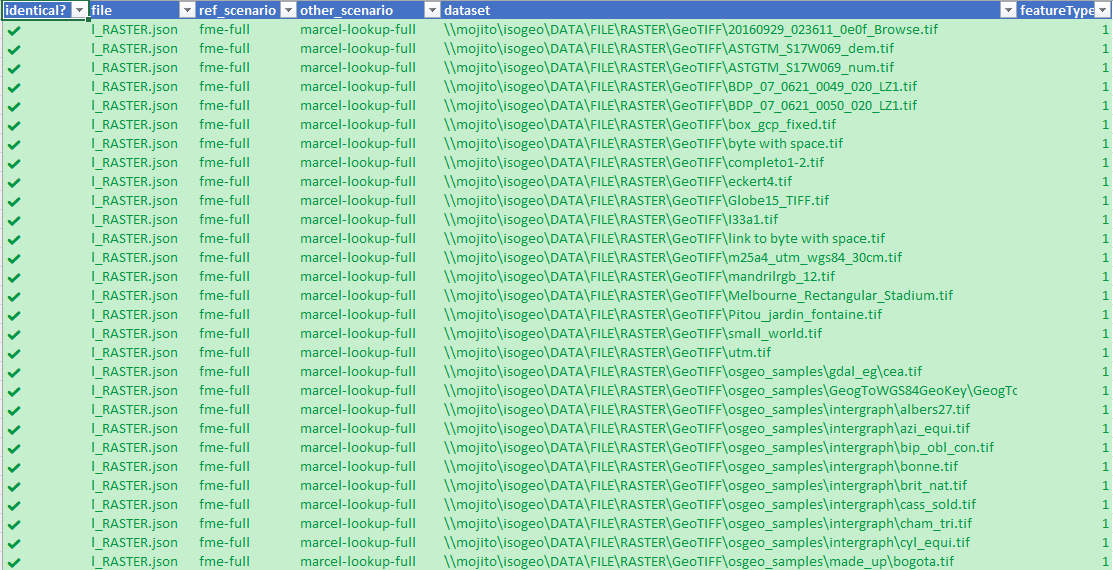
\includegraphics[width=\textwidth]{figures/isogeo/regression_listing.png}
\caption{Test de non-régression sur le listing}
\label{fig:regression_listing}
\end{subfigure}

\medskip

\begin{subfigure}[t]{0.9\textwidth}
\centering
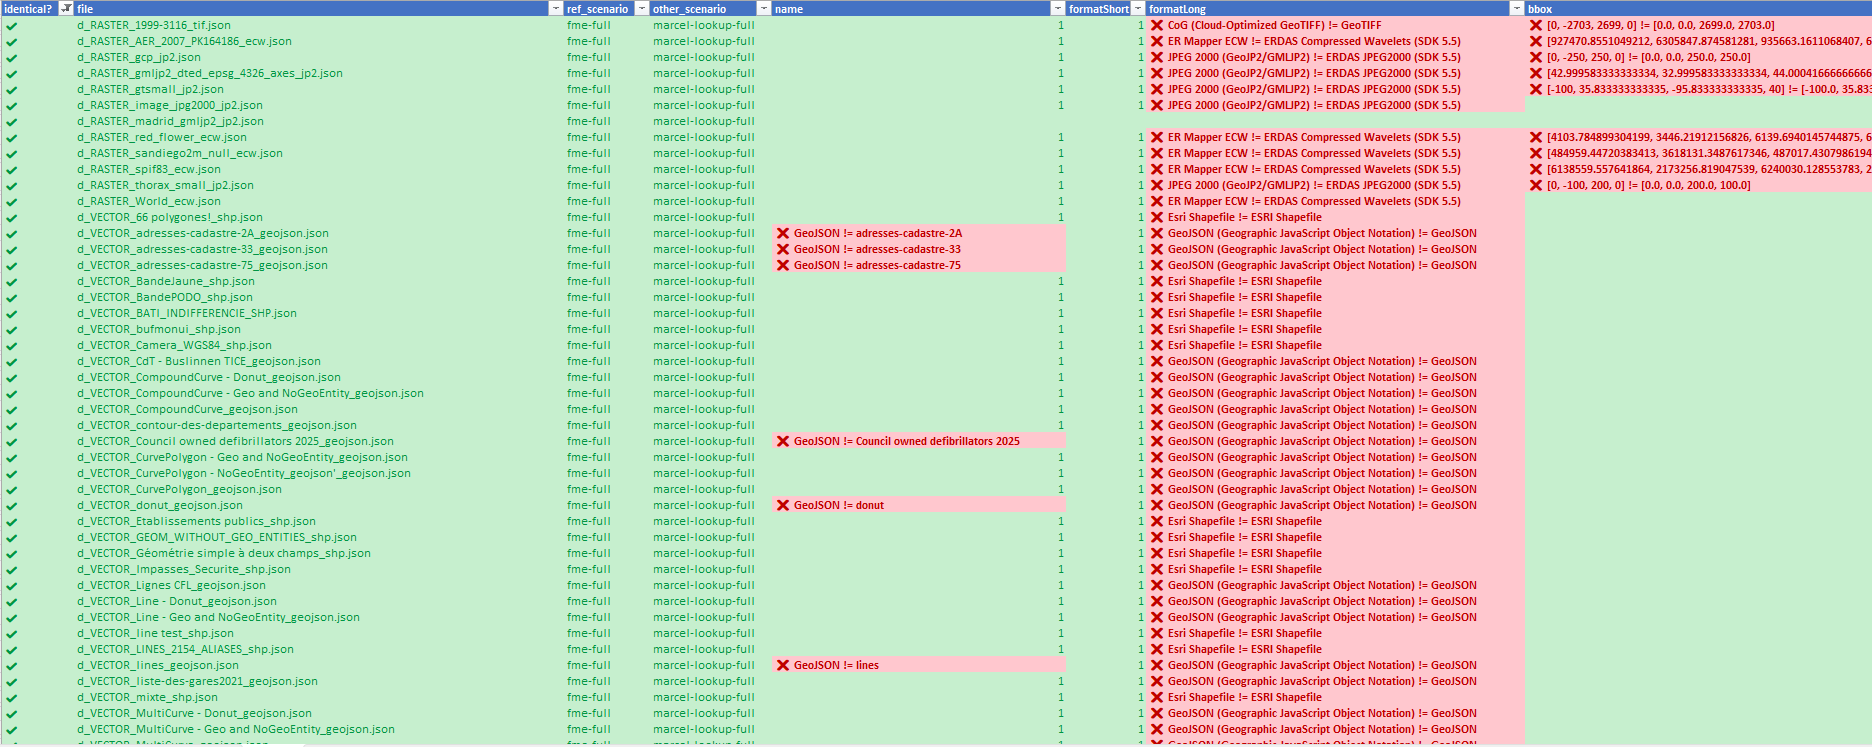
\includegraphics[width=\textwidth]{figures/isogeo/regression_lookup.png}
\caption{Test de non-régression sur le lookup}
\label{fig:regression_lookup}
\end{subfigure}
\caption{Exemples de tests de non-régression}
\label{fig:validation_non_regression}
\end{figure}

La validation ne se limitait pas à constater qu'un test passait ou échouait.
Lorsqu'un écart apparaissait, il devait être analysé afin de déterminer s'il
s'agissait d'une régression, d'un comportement acceptable ou d'une différence à
documenter.

\begin{figure}[H]
\centering
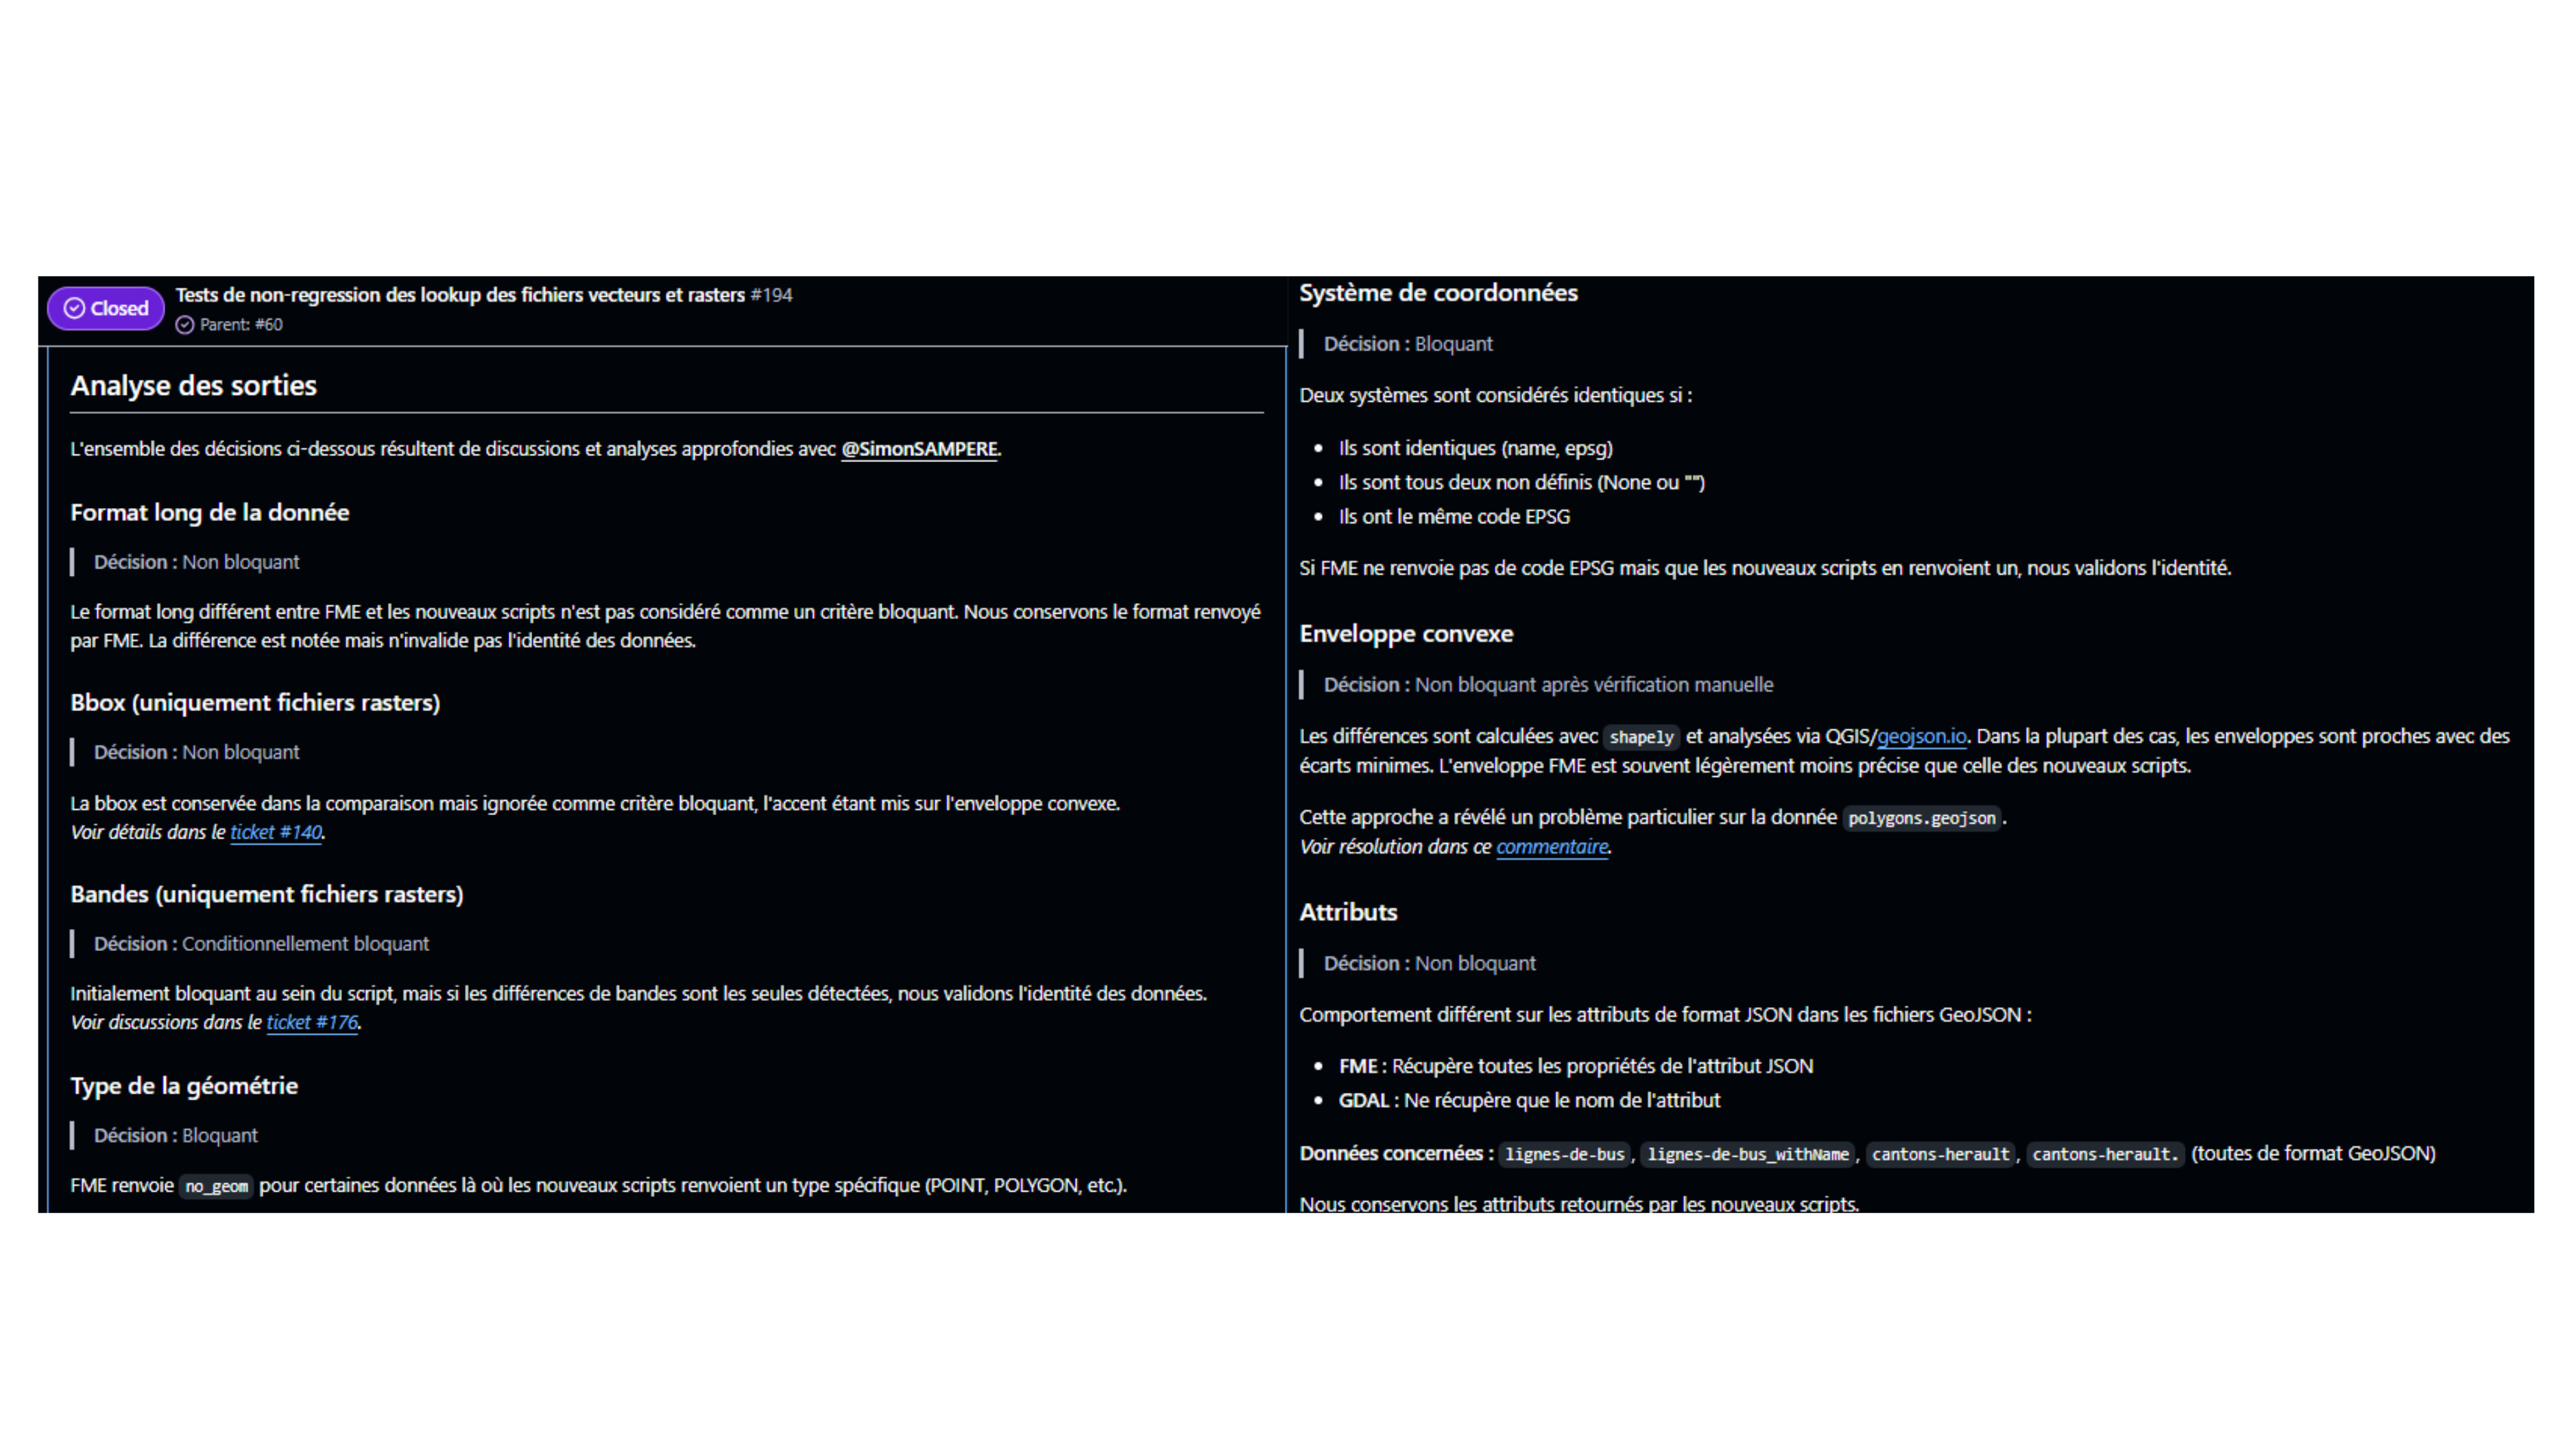
\includegraphics[width=0.92\textwidth]{figures/isogeo/choix_de_validation_des_tests.jpg}
\caption{Méthode de décision utilisée pour valider les tests de non-régression}
\label{fig:choix_validation_tests_non_regression}
\end{figure}

\subsection{Tests d'intégrité de la signature}
\label{subsec:tests_integrite_signature_chapitre_4}

Les tests d'intégrité concernaient la signature. L'objectif était de vérifier
que l'empreinte produite restait stable lorsque la donnée ne changeait pas, mais
qu'elle évoluait dès qu'une modification significative était appliquée.

L'image suivante présente un exemple de résultats obtenus. Pour chaque donnée,
plusieurs scénarios sont exécutés : constance de la signature, modification
attributaire, modification géométrique, changement de structure, changement
spatial ou absence de la donnée. Le résultat attendu est que chaque scénario
soit correctement détecté ou rejeté selon le cas testé.

\begin{figure}[H]
\centering
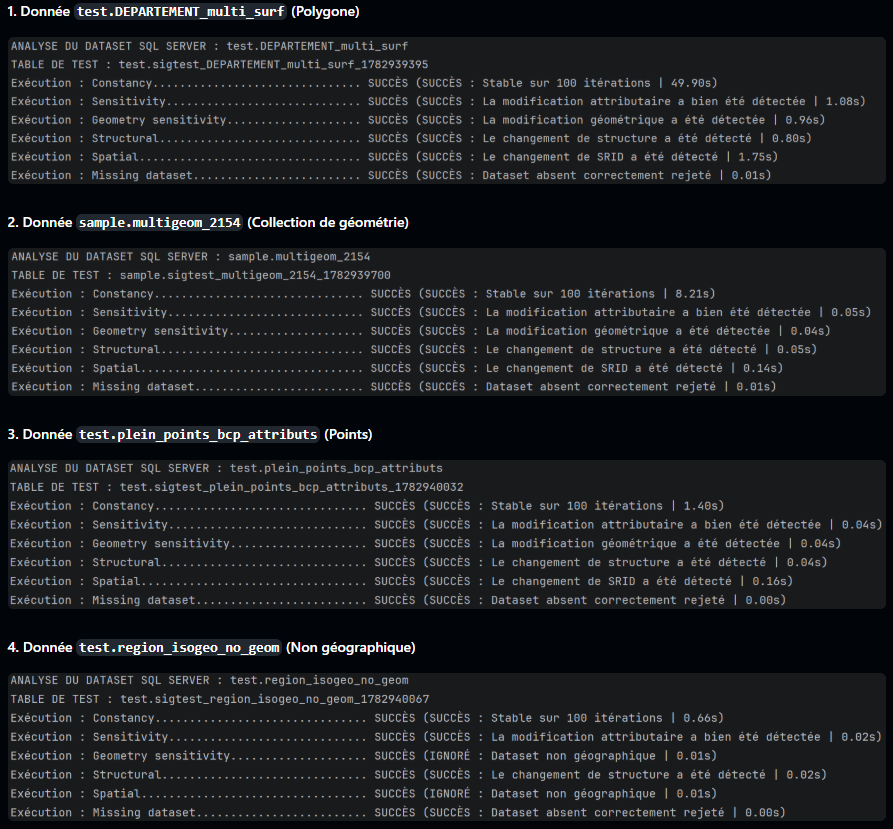
\includegraphics[width=\textwidth]{figures/isogeo/sign_integrity.png}
\caption{Exemple de résultats des tests d'intégrité de la signature}
\label{fig:tests_integrite_signature}
\end{figure}

Les résultats visibles indiquent que les scénarios testés aboutissent au
comportement attendu. La constance montre que la signature reste stable sur
plusieurs exécutions lorsque la donnée n'est pas modifiée. Les tests de
sensibilité confirment ensuite que les modifications attributaires,
géométriques, structurelles ou spatiales sont bien détectées.

L'image montre aussi que les cas particuliers sont pris en compte. Une donnée
non géographique ne déclenche pas de test géométrique, car ce contrôle n'a pas
de sens dans ce contexte. De même, lorsqu'une donnée est absente, le traitement
doit la rejeter correctement au lieu de produire une signature trompeuse. Ces
résultats permettent donc de vérifier que la signature est stable, sensible aux
bons changements et cohérente avec la nature de la donnée analysée.

\subsection{Tests de performance}
\label{subsec:tests_performance_chapitre_4}

Les tests de performance visaient à vérifier le comportement des scripts sur
des volumes de données importants. Ils concernaient l'inventaire, la
documentation et la signature.

Ces tests étaient nécessaires car Scan peut être utilisé sur des environnements
contenant de nombreuses tables, des fichiers volumineux ou des couches avec un
grand nombre d'entités. Un traitement fonctionnel sur un petit jeu de données
peut devenir trop lent ou trop coûteux lorsqu'il est appliqué à un volume plus
important.

Les mesures portaient principalement sur les temps d'exécution et sur les
opérations les plus sensibles. Pour la signature, par exemple, la lecture par
lots permettait de traiter de grandes tables sans charger tout le contenu en
mémoire. Pour la documentation, l'enjeu était de récupérer les métadonnées
utiles sans effectuer des calculs inutilement coûteux.

\begin{figure}[H]
\centering
\fbox{%
\parbox{0.86\textwidth}{%
\centering
\textbf{Figure à mettre}\\[0.25cm]
Quelques résultats de tests de performance sur l'inventaire, la documentation
ou la signature.
}}
\caption{Exemples de résultats de tests de performance}
\label{fig:resultats_tests_performance_a_mettre}
\end{figure}

% =============================================================================
% 4.3 LIMITES RENCONTREES
% =============================================================================

\section{Limites rencontrées}
\label{sec:limites_rencontrees}

La mission a aussi mis en évidence plusieurs limites. Certaines étaient liées
aux formats eux-mêmes, d'autres aux environnements de test ou au packaging.

\subsection{Limites liées aux formats}
\label{subsec:limites_formats}

Tous les formats ne présentaient pas le même niveau de prise en charge. Les
données CAO en sont un bon exemple. Les formats \texttt{DWG} et \texttt{DXF}
proviennent du dessin assisté par ordinateur : ils peuvent contenir des objets
graphiques, du texte ou des éléments de dessin qui ne correspondent pas toujours
à une donnée SIG classique.

La première difficulté a donc été de comprendre les informations réellement
disponibles dans ces fichiers et la manière de les récupérer sans leur donner un
sens géographique qu'elles n'avaient pas forcément. Ce travail d'étude était
nécessaire pour produire des métadonnées fiables et cohérentes avec ce que le
fichier contenait réellement.

Les formats \texttt{SDF} et \texttt{DGN} ont été écartés dans cette première
phase. Leur prise en charge par les bibliothèques étudiées n'était pas
suffisamment fiable et ils étaient moins utilisés par les clients. Ce choix a
permis de concentrer les efforts sur les formats pouvant être traités de manière
plus stable.

\subsection{Limites liées aux environnements de test}
\label{subsec:limites_environnements_test}

La disponibilité des jeux de données variait selon les technologies. Pour
Oracle, des données de test étaient disponibles sur un serveur de l'entreprise.
Pour SQL Server, il a fallu créer un environnement local afin de disposer d'un
jeu de données représentatif.

Cette situation montre qu'une migration ne dépend pas seulement du code. Elle
nécessite aussi des données fiables pour vérifier les résultats. Sans jeux de
tests suffisamment variés, il devient plus difficile d'identifier les écarts, de
tester les cas limites et de mesurer correctement les performances.

\subsection{Limites liées au packaging}
\label{subsec:limites_packaging}

Le packaging sous Windows reste une partie sensible du projet. Les
bibliothèques géospatiales reposent sur des dépendances natives et sur des
données internes, comme celles utilisées par PROJ. Elles doivent être embarquées
correctement avec l'exécutable pour éviter de dépendre de l'environnement local
de la machine.

La mise en place de Docker a permis de rendre la génération plus reproductible,
mais cette étape demande une attention continue. Les versions des bibliothèques,
les chemins internes et les fichiers embarqués doivent rester cohérents pour que
l'exécutable fonctionne de manière stable.

% =============================================================================
% 4.4 APPORTS DE L'ALTERNANCE
% =============================================================================

\section{Apports de l'alternance}
\label{sec:apports_alternance}

Cette mission m'a permis de progresser sur plusieurs dimensions : technique,
méthodologique et professionnelle.

\subsection{Apports techniques}
\label{subsec:apports_techniques}

Sur le plan technique, l'alternance m'a permis de renforcer ma pratique de
Python dans un contexte concret de géomatique. J'ai travaillé sur des formats et
technologies variés : fichiers vectoriels, rasters, GeoPackage, GeoParquet,
CAO, Oracle, SQL Server et nuages de points.

J'ai également approfondi l'utilisation de bibliothèques spécialisées comme
GDAL/OGR, \textit{python-oracledb} ou SQLAlchemy. Ces outils imposent de
comprendre les formats manipulés, leurs limites et les informations qu'ils
permettent réellement d'obtenir.

Cette alternance m'a aussi permis de renforcer ma pratique de Git dans un cadre
professionnel. J'ai appris à organiser mon travail, à versionner correctement mes scripts, à soumettre des
modifications sous forme de Pull Request et à prendre en compte les retours de
revue de code.

Le travail réalisé m'a également sensibilisé à la qualité du code. Il ne
s'agissait pas seulement de produire un script fonctionnel, mais aussi un code
lisible, maintenable, cohérent avec l'existant et suffisamment clair pour être
repris par d'autres développeurs.

Enfin, le travail sur le packaging m'a permis de mieux comprendre les enjeux de
distribution d'une application Python. Une solution doit pouvoir être exécutée
dans un environnement réel, avec des dépendances maîtrisées et un processus de
génération reproductible.

\subsection{Apports méthodologiques}
\label{subsec:apports_methodologiques}

La mission m'a appris à aborder un existant complexe de manière progressive. Il
fallait lire le code déjà présent, comprendre les choix réalisés avant mon
arrivée, documenter ce qui avait été compris et avancer sans rompre le
fonctionnement attendu par Scan.

La méthode de validation a aussi été un apport important. Les tests de
non-régression, les tests d'intégrité et les tests de performance m'ont permis
de mieux structurer mon travail. Ils donnaient un cadre pour vérifier les
résultats et pour discuter les écarts avec l'équipe.

La revue de code a également joué un rôle central. Les retours de mon tuteur
permettaient d'améliorer les scripts, de justifier certains choix et de
progresser vers une solution plus robuste.

\subsection{Apports professionnels}
\label{subsec:apports_professionnels}

Sur le plan professionnel, cette alternance a d'abord été une expérience
d'intégration réussie au sein de l'entreprise. L'humain y occupe une place
importante et les valeurs de collaboration, d'écoute et de confiance sont
réellement présentes dans le quotidien de travail.

Cette intégration s'est ensuite construite plus précisément au sein de l'équipe
Produit. Les points de suivi, les stand-up meetings, les revues de sprint et les
échanges techniques m'ont aidé à mieux comprendre l'organisation du travail en
entreprise et la manière dont un produit logiciel évolue collectivement.

J'ai aussi gagné en autonomie. Les tâches confiées demandaient de chercher des
solutions, de comparer plusieurs approches, de documenter les résultats et de
présenter les choix effectués. Cette progression s'est faite avec un
accompagnement régulier, mais aussi avec une responsabilité croissante dans la
conduite des développements.

% =============================================================================
% 4.5 PERSPECTIVES ET RECOMMANDATIONS
% =============================================================================

\section{Perspectives et recommandations}
\label{sec:perspectives_recommandations}

Les travaux réalisés constituent une étape dans la migration progressive des
traitements de Scan. Ils ouvrent plusieurs perspectives pour la suite du
projet.

\subsection{Poursuite de la migration}
\label{subsec:poursuite_migration}

La première perspective consiste à poursuivre la migration sur les traitements
encore en cours ou non couverts. Les nuages de points devront notamment être
approfondis afin de choisir l'approche la plus adaptée entre les solutions
étudiées.

La migration pourra également être étendue à d'autres formats ou technologies
selon les besoins du produit et les usages des clients. Cette poursuite devra
rester progressive, car chaque format apporte ses propres contraintes.

\subsection{Enrichissement des métadonnées}
\label{subsec:enrichissement_metadonnees}

Une autre perspective concerne l'enrichissement des métadonnées produites par
Scan. Les traitements Python et les bibliothèques utilisées permettent déjà de
récupérer de nombreuses informations sur les ressources analysées. La suite
pourrait consister à exploiter davantage ces possibilités afin de produire des
fiches plus complètes.

Une piste complémentaire serait d'étudier l'utilisation de modèles
d'intelligence artificielle pour générer automatiquement des suggestions de
descriptions pour certaines métadonnées. L'objectif ne serait pas de remplacer
la validation humaine, mais d'aider au remplissage manuel des champs et de
rendre le catalogage moins chronophage.

Cette approche devrait d'abord rester dans un cadre de recherche et
développement. Elle nécessiterait de vérifier la qualité des suggestions, leur
cohérence avec les données analysées et leur intérêt réel pour les utilisateurs
de Scan.


% =============================================================================
% 4.6 CONCLUSION GENERALE
% =============================================================================

\section{Conclusion}
\label{sec:conclusion_generale}

Ce rapport a présenté le travail réalisé pendant mon alternance autour de la
migration progressive des traitements de Scan vers une solution Python plus
autonome. Les développements menés ont contribué à faire avancer cette
migration sur plusieurs formats et technologies, avec des niveaux d'avancement
différents selon les cas : documentation, inventaire, signature ou étude
préparatoire.

La validation a constitué un point essentiel du travail. Les tests de
non-régression ont permis de comparer les nouvelles sorties Python avec les
références existantes lorsque cela était possible. Les tests d'intégrité ont
servi à vérifier la fiabilité des signatures. Les tests de performance ont
permis de contrôler le comportement des scripts sur des volumes plus importants.

La mission a aussi montré que la migration ne se résume pas à remplacer un outil
par un autre. Elle demande de comprendre les formats, de gérer leurs limites, de
préparer des environnements de test fiables et de s'assurer que les traitements
restent compatibles avec les besoins de Scan.

Au-delà des résultats techniques, cette alternance m'a permis de progresser dans
un contexte professionnel exigeant, au contact d'une équipe Produit et de
méthodes de développement structurées. Les perspectives restent ouvertes,
notamment autour de la poursuite de la migration, du renforcement des tests et
de la stabilisation du processus de génération de l'exécutable.
